% Author: Izaak Neutelings (July 2020)
\documentclass[border=3pt,tikz]{standalone}
\usepackage{amsmath} % for \;
\usepackage{tikz}
\usepackage{xcolor}
\colorlet{myblue}{blue!70!black}
\colorlet{mylightblue}{blue!10}
\colorlet{branch}{green!30!black}
\colorlet{evolcol}{green!50!black}
\colorlet{natalcol}{red!50!white!60!black}
\colorlet{hormcol}{orange!70!black}
\colorlet{ethcol}{yellow!80!black}
\colorlet{stimcol}{red!80!black}
\colorlet{neurcol}{blue!80!black}
\tikzset{>=latex} % for LaTeX arrow head
\usetikzlibrary{tikzmark} % for subnode
\usetikzlibrary{decorations.pathreplacing} % for curly braces

\begin{document}


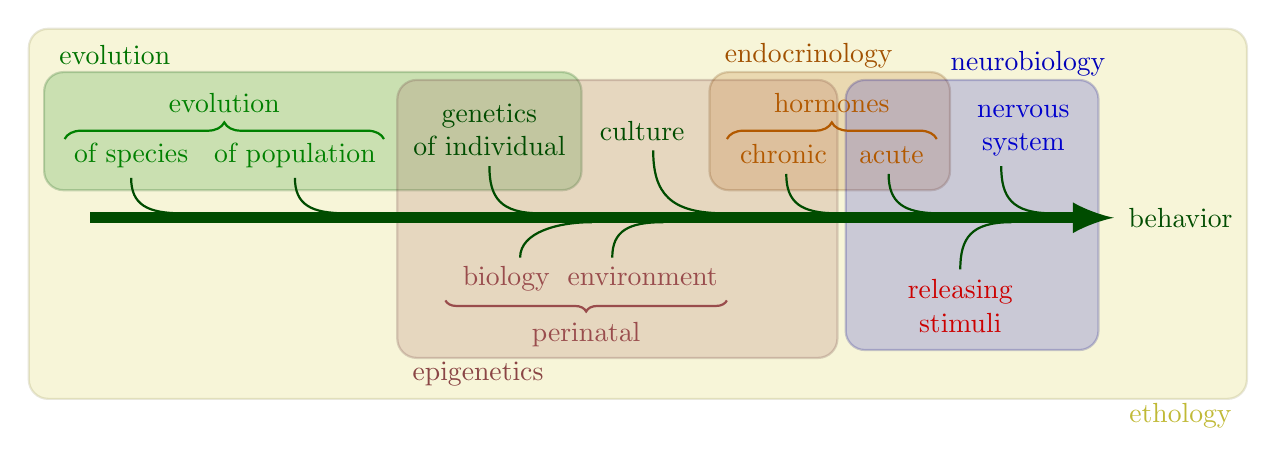
\begin{tikzpicture}[xscale=1.3]
  \def\t{0.056} % stem half-thickness
    
  % GROUPS
  \draw[thick,ethcol!60!black,fill=ethcol!90,rounded corners=7,opacity=0.2]
    (-0.6,-2.3) rectangle (11.3,2.4);
  \draw[thick,evolcol!60!black,fill=evolcol!90,rounded corners=7,opacity=0.2]
    (-0.45,0.35) rectangle (4.8,1.85);
  \draw[thick,natalcol!60!black,fill=natalcol!90,rounded corners=7,opacity=0.2]
    (3.0,-1.78) rectangle (7.3,1.75);
  \draw[thick,hormcol!60!black,fill=hormcol!90,rounded corners=7,opacity=0.2]
    (6.05,1.85) rectangle (8.4,0.35);
  %\draw[thick,ethcol!60!black,fill=ethcol!90,rounded corners=7,opacity=0.2]
  %  (7.4,-1.65) rectangle (11.3,1.75);
  %\draw[thick,neurcol!60!black,fill=neurcol!90,rounded corners=7,opacity=0.2]
  %  (9.85,1.75) rectangle (7.35,0.43);
  \draw[thick,neurcol!60!black,fill=neurcol!90,rounded corners=7,opacity=0.2]
    (7.38,-1.68) rectangle (9.85,1.75);
  \node[evolcol!90!black,below=2,above right=2] at (-0.45,1.82) {evolution};
  \node[natalcol!90!black,above=4,below right=2] at (3,-1.78) {epigenetics};
  \node[hormcol!90!black,below=3,above right=2] at (6.05,1.82) {endocrinology};
  %\node[ethcol!90!black,above=4,below right=2] at (7.4,-1.65) {ethology};
  \node[ethcol!90!black,above=4,below left=2] at (11.3,-2.3) {ethology};
  \node[neurcol!90!black,below=4,right=8,above left=2] at (9.85,1.75) {neurobiology};
  
  % BRANCHES
  \draw[->,branch,line width=4] (0,0) -- (10,0) node[right] {behavior};
  \draw[branch,thick] (0.9, \t) to[out=180,in=-90,looseness=1.3]++ (-0.5, 0.45)
    node[evolcol,above] {of species};
  \draw[branch,thick] (2.5, \t) to[out=180,in=-90,looseness=1.3]++ (-0.5, 0.45)
    node[evolcol,above] {of population};
  \draw[branch,thick] (4.4, \t) to[out=180,in=-90,looseness=1.3]++ (-0.5, 0.6)
    node[above,align=center] {genetics\\of individual};
  \draw[branch,thick] (4.9,-\t) to[out=180,in= 90,looseness=1.0]++ (-0.7,-0.45)
    node[natalcol,left=5,below=-2] {\strut biology};
  \draw[branch,thick] (5.6,-\t) to[out=180,in= 90,looseness=1.3]++ (-0.5,-0.45)
    node[natalcol,right=11,below=-2] {\strut environment};
  \draw[branch,thick] (6.2, \t) to[out=180,in=-90,looseness=1.3]++ (-0.7, 0.8)
    node[left=4,above] {culture};
  \draw[branch,thick] (7.3, \t) to[out=180,in=-90,looseness=1.3]++ (-0.5, 0.5)
    node[hormcol,left=1,above] {chronic};
  \draw[branch,thick] (8.3, \t) to[out=180,in=-90,looseness=1.3]++ (-0.5, 0.5)
    node[hormcol,right=1,above] {acute};
  \draw[branch,thick] (9.0,-\t) to[out=180,in= 90,looseness=1.3]++ (-0.5,-0.60)
    node[stimcol,below,align=center] {releasing\\stimuli};
  \draw[branch,thick] (9.4, \t) to[out=180,in=-90,looseness=1.3]++ (-0.5, 0.60)
    node[neurcol,right=8,above,align=center] {nervous\\system};
  
  % BRANCHES
  \draw[thick,evolcol,decorate,decoration={brace,amplitude=6}]
    (-0.25,1.0) --++ (3.12,0) node[midway,above=6] {evolution};
  \draw[thick,natalcol,decorate,decoration={brace,amplitude=4}]
    (6.22,-1.05) --++ (-2.75,0) node[midway,below=4] {perinatal};
  \draw[thick,hormcol,decorate,decoration={brace,amplitude=6}]
    (6.22,1.0) --++ (2.05,0) node[midway,above=6] {hormones};

\end{tikzpicture}



\end{document}